\documentclass[10pt,a4paper]{article}
\usepackage[margin=13mm]{geometry}
\usepackage[T1]{fontenc}
\usepackage{graphicx,amsmath,booktabs,array}
\usepackage[hidelinks]{hyperref}
\setlength{\parindent}{0pt}
\setlength{\parskip}{2.5pt}
\setlength{\abovedisplayskip}{5pt}
\setlength{\belowdisplayskip}{5pt}
\pagestyle{plain}
\graphicspath{{figures/}}
\makeatletter
\renewcommand\section{\@startsection{section}{1}{0pt}{7pt}{3pt}{\large\bfseries}}
\makeatother

\begin{document}
\begin{center}
  {\Large\bfseries Image Restoration with Shared NAFNet and D4 Fine-Tuning}
\end{center}
\vspace{-8pt}

\section{Method}
The task is to recover clean RGB images from blurred, noisy inputs without
knowing the corruption parameters. We adapt the NAFNet architecture and gated
restoration blocks of Chen et al.~\cite{chen2022nafnet}, using a residual
encoder--decoder with skip connections, widths $32/64/128$ and block depths
$2/2/7/2/2$. To meet the storage budget, our implementation shares convolutions
\emph{within each network stage}; normalization and residual gates remain
independent at each depth. This gives \textbf{286,563 trainable parameters} and
\textbf{286,942/300,000 stored ONNX tensor elements}. The self-contained
opset-18 graph has FP32 input/output $[1,3,384,384]$ and clips outputs to $[0,1]$.

Only the supplied 1,200 training pairs are used: no external images or
pretrained weights. We train on synchronized $256\!\times\!256$ crops with
random quarter-turn rotations and horizontal flips. All 120 validation pairs
retain the supplied split and full $384\!\times\!384$ resolution.
The objective is mean \emph{per-image} log-MSE:
\[
 m_b=\frac{1}{CHW}\lVert\hat y_b-y_b\rVert_2^2,
 \qquad \mathcal L=\frac1B\sum_{b=1}^{B}\ln\!\bigl(\max(m_b,10^{-12})\bigr).
\]
Scratch/native use $\hat y=f_\theta(x)$. The D4 stage adapts the geometric
self-ensemble used for inference by Lim et al.~\cite{lim2017edsr}:
$\hat y=\tfrac18\sum_{t\in D_4}t^{-1}f_\theta(tx)$. Eight rotated/reflected
views share weights and are inverse-transformed before averaging. Here we
also \emph{train through this average}, computing the loss after averaging.
This training adaptation and within-stage convolution sharing are project
choices. Training outputs are unclipped; export uses the same D4 average
with final clipping.

\section{Training}
The submitted checkpoint follows the three-stage schedule below.
\begin{center}
\small
\renewcommand{\arraystretch}{1.1}
\begin{tabular}{@{}lcccccc@{}}
\toprule
Stage & Epochs & Cosine $T_{\max}$ & Initial LR $\to\eta_{\min}$ & Batch & Seed & Precision \\
\midrule
Scratch & 150 & 300 & $10^{-3}\to10^{-5}$ & 4 & 42 & FP32 \\
Native & 300 & 300 & $5\!\times\!10^{-4}\to2\!\times\!10^{-6}$ & 4 & 42 & FP32 \\
D4 & 40 & 40 & $7.5\!\times\!10^{-5}\to10^{-6}$ & 2 & 4246 & BF16 \\
\bottomrule
\end{tabular}
\end{center}
\vspace{-6pt}

All stages use AdamW ($\beta=(0.9,0.999)$, $\epsilon=10^{-8}$,
weight decay $10^{-4}$), gradient-norm clipping at~1 and EMA decay~0.999.
Cosine scheduling steps after each epoch's validation. Scratch was initially
planned for 300 epochs, then truncated to 150 as an experimental budget
choice, retaining the original cosine schedule. Native loads scratch
epoch~150 EMA; D4 loads native \textbf{epoch~300 EMA}.
Only EMA weights transfer: each stage resets optimizer, scheduler and seeded
RNG. D4 also changes the training batch size from 4 to~2.
The strict run uses deterministic kernels and seeded shuffling, with TF32 and
compilation disabled. BF16 is used only for the D4 forward pass; master weights,
loss, EMA and validation remain FP32. We export \textbf{D4 epoch~39 EMA}.

\section{Results}
Official CPU ONNX scoring averages per-image full-image RGB PSNR over all
120 validation images, using float64 scoring and no border crop.
The starter score is the reference reported in the assignment README.
\begin{center}
\small
\renewcommand{\arraystretch}{1.1}
\begin{tabular}{@{}lc@{}}
\toprule
Method & Mean PSNR (dB) \\
\midrule
Degraded input & 29.7931 \\
Starter CNN & 31.74 \\
Shared NAFNet + D4 (ours) & \textbf{35.5189} \\
\bottomrule
\end{tabular}
\end{center}
\vspace{-7pt}

\begin{center}
  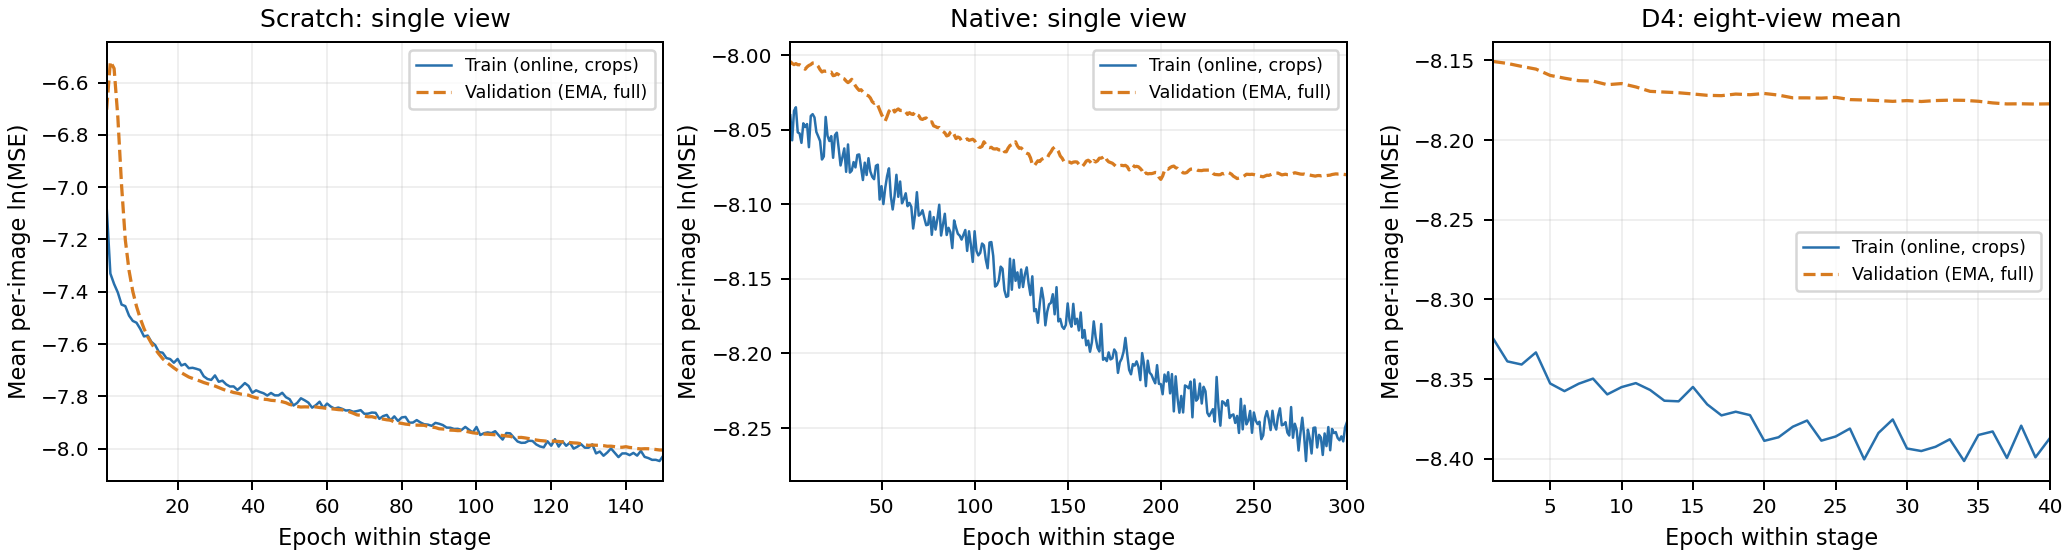
\includegraphics[width=0.90\linewidth,height=0.165\textheight,keepaspectratio]{loss.png}
\end{center}
\vspace{-7pt}
{\small\textbf{Training curves.} Each panel uses local epochs and its own
vertical range, with the same mean per-image $\ln(\mathrm{MSE})$ objective:
solid training, dashed EMA validation.
Stages are not joined. The D4 boundary reflects a new eight-view forward
pass, smaller batch and reset optimizer/scheduler, \emph{not missing epochs}.}

\newpage
\section*{Qualitative results}
Two fixed validation examples show degraded input, our restoration and the
clean target. The matching central $96\!\times\!96$ crop is enlarged below each
full image; PSNR labels use the full-image metric.

\begin{center}
  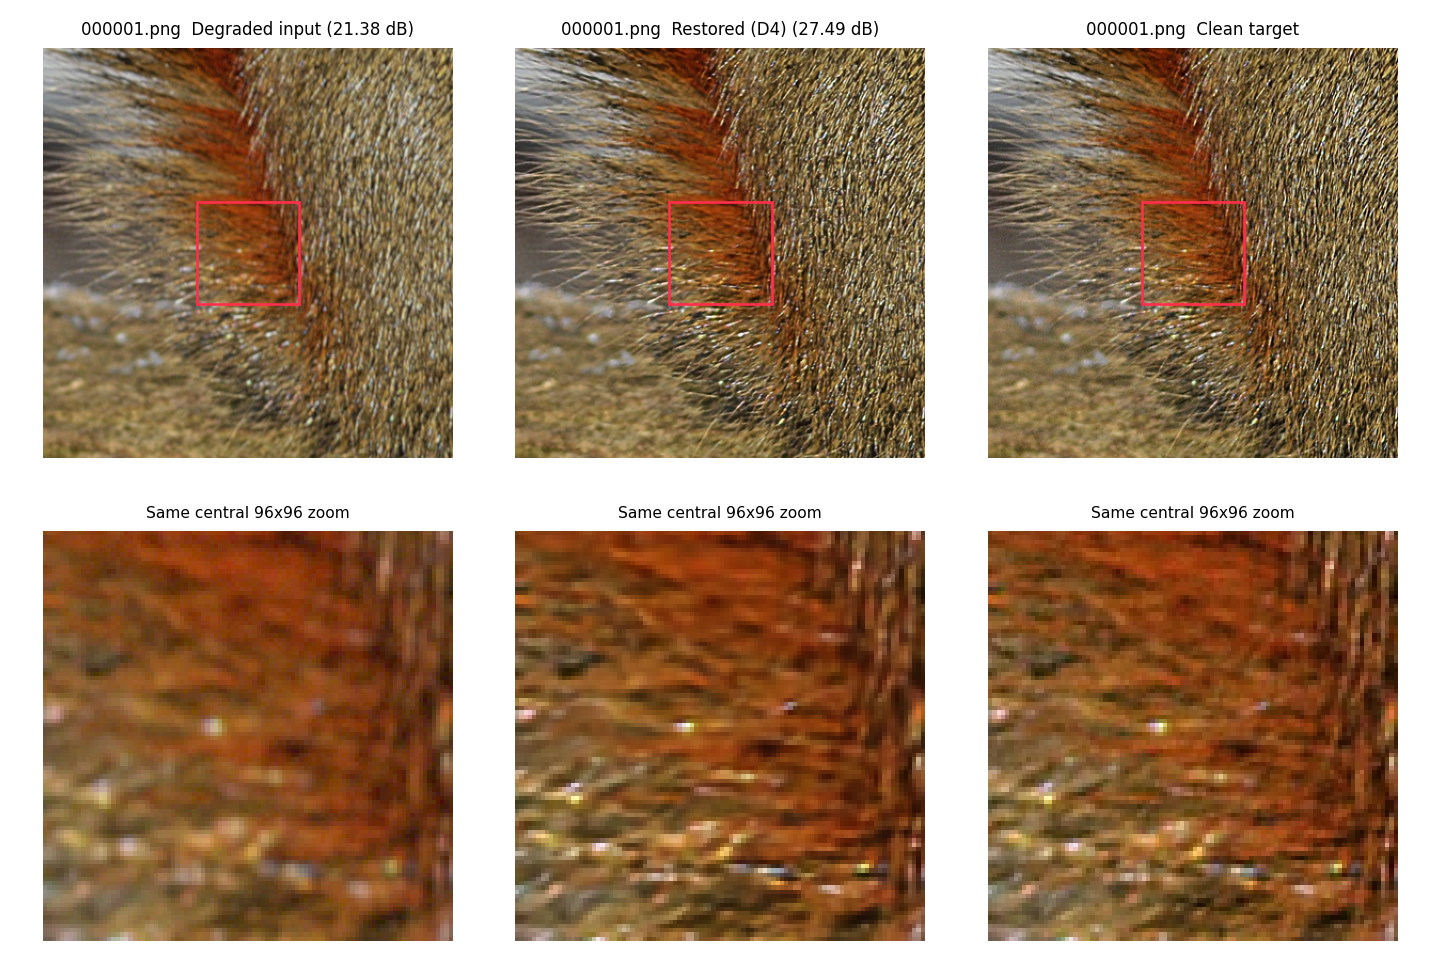
\includegraphics[width=0.90\linewidth,height=0.34\textheight,keepaspectratio]{comparison_1.png}\\[3pt]
  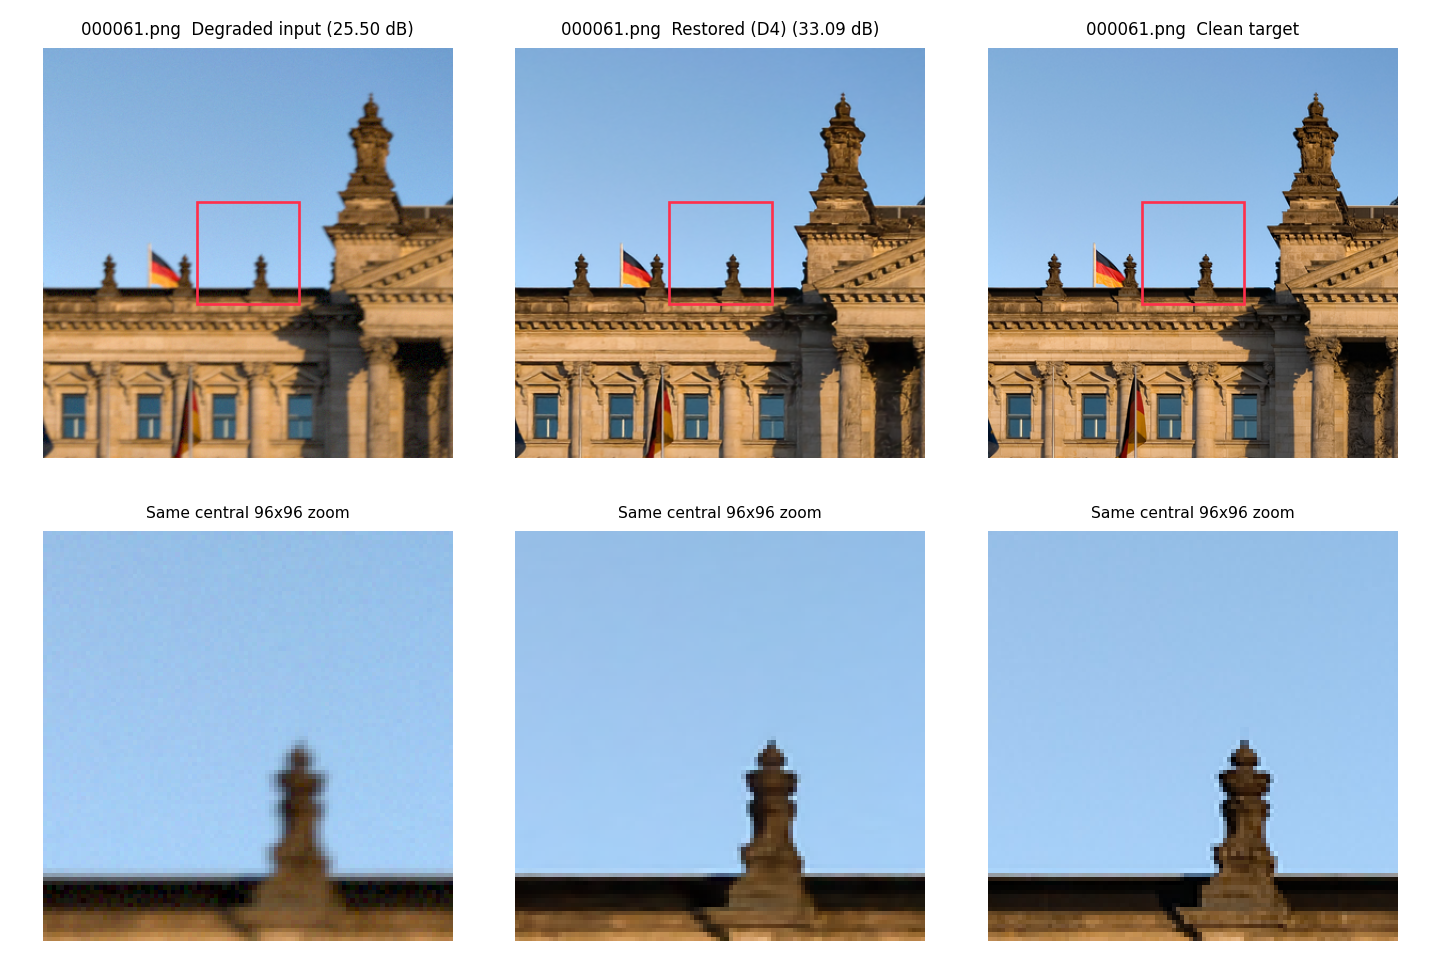
\includegraphics[width=0.90\linewidth,height=0.34\textheight,keepaspectratio]{comparison_2.png}
\end{center}
\vspace{-5pt}

{\small
\begin{thebibliography}{9}
\setlength{\itemsep}{1pt}
\setlength{\parskip}{0pt}
\bibitem{chen2022nafnet}
Liangyu Chen, Xiaojie Chu, Xiangyu Zhang, and Jian Sun.
\emph{Simple Baselines for Image Restoration}. ECCV, 2022.
\href{https://arxiv.org/abs/2204.04676}{arXiv:2204.04676}.
\bibitem{lim2017edsr}
Bee Lim, Sanghyun Son, Heewon Kim, Seungjun Nah, and Kyoung Mu Lee.
\emph{Enhanced Deep Residual Networks for Single Image Super-Resolution}.
CVPR Workshops, 2017.
\href{https://arxiv.org/abs/1707.02921}{arXiv:1707.02921}.
\end{thebibliography}}
\end{document}
